% SUBJECT gallery (P1 analog: p1_fig8). AUTO-GENERATED by no_upload/gen_subject_gallery_p3.py.
% Tiles are real subject/scene figures cropped from each benchmark's arXiv paper;
% per-panel provenance in Table~\ref{tab:panel_provenance}. Grouped by evaluation lane.
\begin{figure*}[p]
\centering
\definecolor{sgClosed}{HTML}{1E8449}\definecolor{sgWM}{HTML}{C2185B}\definecolor{sgBridge}{HTML}{7C3AED}%
\resizebox{\textwidth}{!}{%
\begin{tikzpicture}[x=1cm,y=1cm]
\fill[black!88] (0,0) rectangle (13.80,-0.72);
\node[anchor=west,text=white,font=\large\bfseries,inner sep=0] at (0.16,-0.36) {Benchmarks across the surveyed corpus};
\node[anchor=east,text=white!70,font=\scriptsize,inner sep=0] at (13.64,-0.36) {vector, zoomable, per-panel arXiv links};
\fill[sgClosed!78!black] (0,-0.720) rectangle (13.80,-1.220);
\node[anchor=west,text=white,font=\footnotesize\bfseries,inner sep=0] at (0.12,-0.970) {CLOSED-LOOP task-success suites};
\node[anchor=north west,inner sep=0] at (0.060,-1.290) {\href{https://arxiv.org/abs/1912.01734}{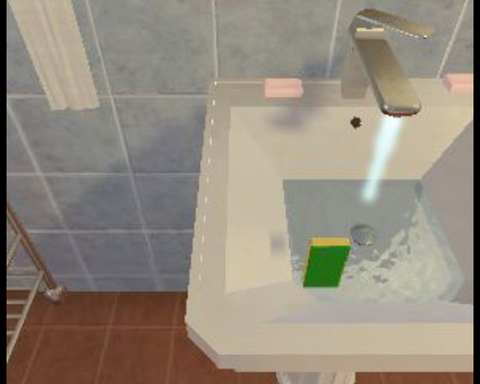
\includegraphics[width=2.660cm,height=2.128cm]{figures/img/subject_tiles/alfred.png}}};
\draw[black!35,line width=0.35pt] (0.060,-1.290) rectangle (2.720,-3.418);
\node[anchor=north west,text=ACMDarkBlue,font=\scriptsize,inner sep=0] at (0.080,-3.438) {\href{https://arxiv.org/abs/1912.01734}{ALFRED}};
\node[anchor=north west,text=black!55,font=\tiny,inner sep=0] at (0.080,-3.668) {\href{https://arxiv.org/abs/1912.01734}{arXiv:1912.01734}};
\node[anchor=north west,inner sep=0] at (2.770,-1.290) {\href{https://arxiv.org/abs/2403.09227}{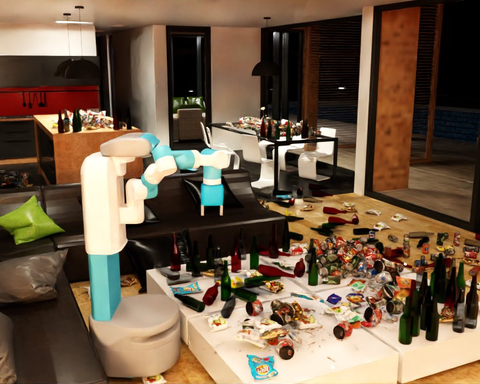
\includegraphics[width=2.660cm,height=2.128cm]{figures/img/subject_tiles/behavior1k.png}}};
\draw[black!35,line width=0.35pt] (2.770,-1.290) rectangle (5.430,-3.418);
\node[anchor=north west,text=ACMDarkBlue,font=\scriptsize,inner sep=0] at (2.790,-3.438) {\href{https://arxiv.org/abs/2403.09227}{BEHAVIOR-1K}};
\node[anchor=north west,text=black!55,font=\tiny,inner sep=0] at (2.790,-3.668) {\href{https://arxiv.org/abs/2403.09227}{arXiv:2403.09227}};
\node[anchor=north west,inner sep=0] at (5.480,-1.290) {\href{https://arxiv.org/abs/2112.03227}{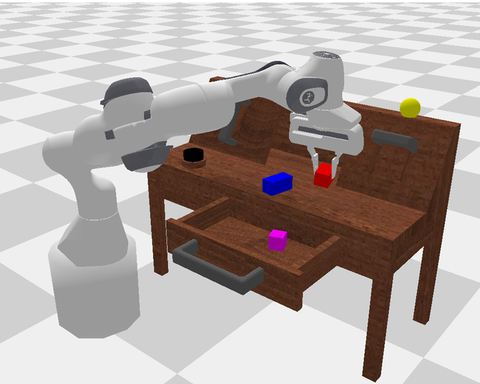
\includegraphics[width=2.660cm,height=2.128cm]{figures/img/subject_tiles/calvin.png}}};
\draw[black!35,line width=0.35pt] (5.480,-1.290) rectangle (8.140,-3.418);
\node[anchor=north west,text=ACMDarkBlue,font=\scriptsize,inner sep=0] at (5.500,-3.438) {\href{https://arxiv.org/abs/2112.03227}{CALVIN}};
\node[anchor=north west,text=black!55,font=\tiny,inner sep=0] at (5.500,-3.668) {\href{https://arxiv.org/abs/2112.03227}{arXiv:2112.03227}};
\node[anchor=north west,inner sep=0] at (8.190,-1.290) {\href{https://arxiv.org/abs/2410.01345}{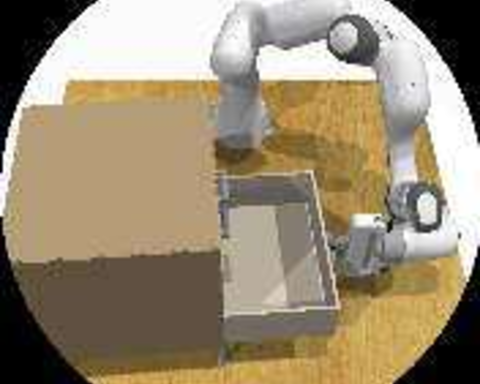
\includegraphics[width=2.660cm,height=2.128cm]{figures/img/subject_tiles/gembench.png}}};
\draw[black!35,line width=0.35pt] (8.190,-1.290) rectangle (10.850,-3.418);
\node[anchor=north west,text=ACMDarkBlue,font=\scriptsize,inner sep=0] at (8.210,-3.438) {\href{https://arxiv.org/abs/2410.01345}{GemBench}};
\node[anchor=north west,text=black!55,font=\tiny,inner sep=0] at (8.210,-3.668) {\href{https://arxiv.org/abs/2410.01345}{arXiv:2410.01345}};
\node[anchor=north west,inner sep=0] at (10.900,-1.290) {\href{https://arxiv.org/abs/2302.04659}{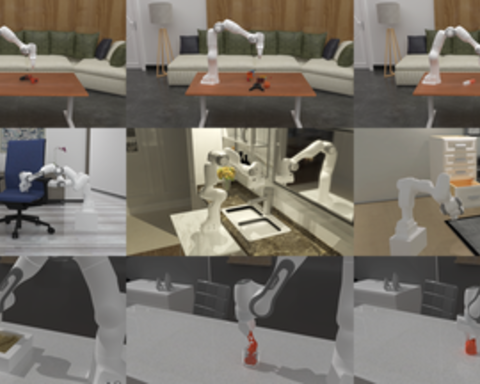
\includegraphics[width=2.660cm,height=2.128cm]{figures/img/subject_tiles/maniskill2.png}}};
\draw[black!35,line width=0.35pt] (10.900,-1.290) rectangle (13.560,-3.418);
\node[anchor=north west,text=ACMDarkBlue,font=\scriptsize,inner sep=0] at (10.920,-3.438) {\href{https://arxiv.org/abs/2302.04659}{ManiSkill2}};
\node[anchor=north west,text=black!55,font=\tiny,inner sep=0] at (10.920,-3.668) {\href{https://arxiv.org/abs/2302.04659}{arXiv:2302.04659}};
\node[anchor=north west,inner sep=0] at (0.060,-4.048) {\href{https://arxiv.org/abs/1910.10897}{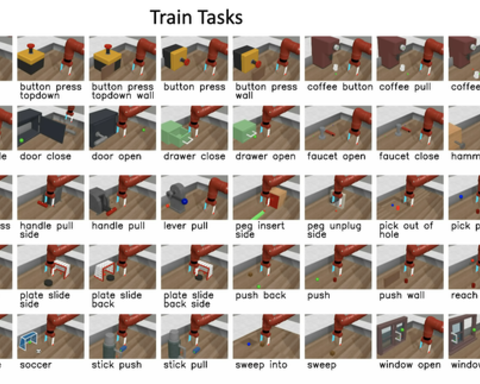
\includegraphics[width=2.660cm,height=2.128cm]{figures/img/subject_tiles/metaworld.png}}};
\draw[black!35,line width=0.35pt] (0.060,-4.048) rectangle (2.720,-6.176);
\node[anchor=north west,text=ACMDarkBlue,font=\scriptsize,inner sep=0] at (0.080,-6.196) {\href{https://arxiv.org/abs/1910.10897}{Meta-World}};
\node[anchor=north west,text=black!55,font=\tiny,inner sep=0] at (0.080,-6.426) {\href{https://arxiv.org/abs/1910.10897}{arXiv:1910.10897}};
\node[anchor=north west,inner sep=0] at (2.770,-4.048) {\href{https://arxiv.org/abs/2406.02523}{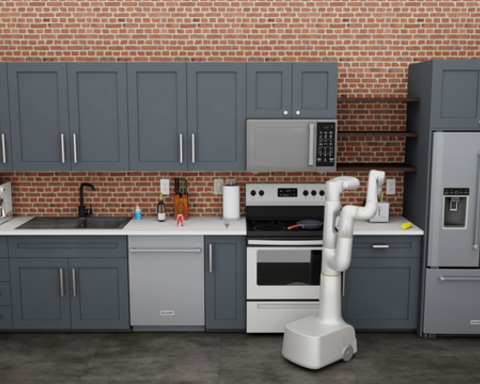
\includegraphics[width=2.660cm,height=2.128cm]{figures/img/subject_tiles/robocasa.png}}};
\draw[black!35,line width=0.35pt] (2.770,-4.048) rectangle (5.430,-6.176);
\node[anchor=north west,text=ACMDarkBlue,font=\scriptsize,inner sep=0] at (2.790,-6.196) {\href{https://arxiv.org/abs/2406.02523}{RoboCasa}};
\node[anchor=north west,text=black!55,font=\tiny,inner sep=0] at (2.790,-6.426) {\href{https://arxiv.org/abs/2406.02523}{arXiv:2406.02523}};
\node[anchor=north west,inner sep=0] at (5.480,-4.048) {\href{https://arxiv.org/abs/2306.03310}{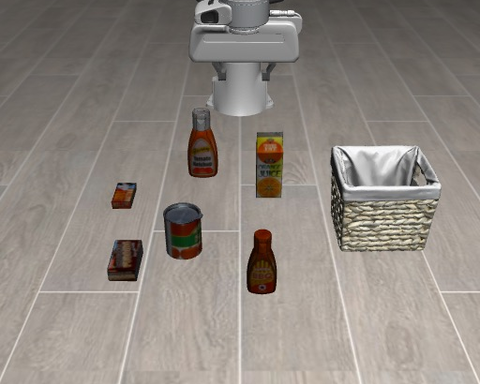
\includegraphics[width=2.660cm,height=2.128cm]{figures/img/subject_tiles/libero.png}}};
\draw[black!35,line width=0.35pt] (5.480,-4.048) rectangle (8.140,-6.176);
\node[anchor=north west,text=ACMDarkBlue,font=\scriptsize,inner sep=0] at (5.500,-6.196) {\href{https://arxiv.org/abs/2306.03310}{LIBERO}};
\node[anchor=north west,text=black!55,font=\tiny,inner sep=0] at (5.500,-6.426) {\href{https://arxiv.org/abs/2306.03310}{arXiv:2306.03310}};
\node[anchor=north west,inner sep=0] at (8.190,-4.048) {\href{https://arxiv.org/abs/2412.18194}{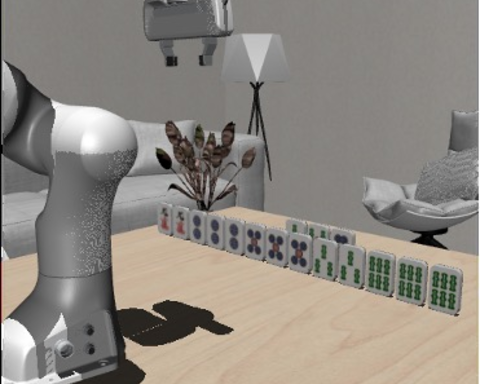
\includegraphics[width=2.660cm,height=2.128cm]{figures/img/subject_tiles/vlabench.png}}};
\draw[black!35,line width=0.35pt] (8.190,-4.048) rectangle (10.850,-6.176);
\node[anchor=north west,text=ACMDarkBlue,font=\scriptsize,inner sep=0] at (8.210,-6.196) {\href{https://arxiv.org/abs/2412.18194}{VLABench}};
\node[anchor=north west,text=black!55,font=\tiny,inner sep=0] at (8.210,-6.426) {\href{https://arxiv.org/abs/2412.18194}{arXiv:2412.18194}};
\node[anchor=north west,inner sep=0] at (10.900,-4.048) {\href{https://arxiv.org/abs/2310.13724}{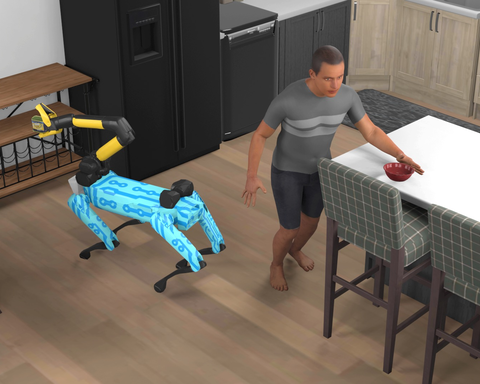
\includegraphics[width=2.660cm,height=2.128cm]{figures/img/subject_tiles/habitat30.png}}};
\draw[black!35,line width=0.35pt] (10.900,-4.048) rectangle (13.560,-6.176);
\node[anchor=north west,text=ACMDarkBlue,font=\scriptsize,inner sep=0] at (10.920,-6.196) {\href{https://arxiv.org/abs/2310.13724}{Habitat 3.0}};
\node[anchor=north west,text=black!55,font=\tiny,inner sep=0] at (10.920,-6.426) {\href{https://arxiv.org/abs/2310.13724}{arXiv:2310.13724}};
\fill[sgWM!78!black] (0,-6.906) rectangle (13.80,-7.406);
\node[anchor=west,text=white,font=\footnotesize\bfseries,inner sep=0] at (0.12,-7.156) {OPEN-LOOP world-model \& video-generation evaluation};
\node[anchor=north west,inner sep=0] at (0.060,-7.476) {\href{https://arxiv.org/abs/2410.15461}{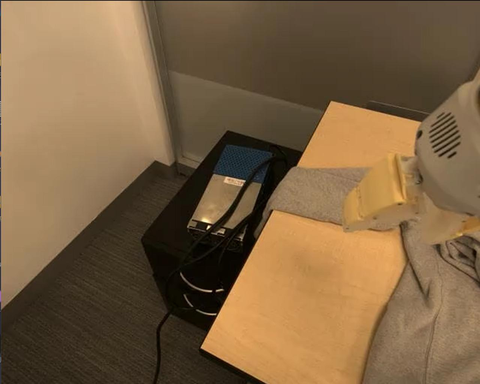
\includegraphics[width=2.660cm,height=2.128cm]{figures/img/subject_tiles/evabench.png}}};
\draw[black!35,line width=0.35pt] (0.060,-7.476) rectangle (2.720,-9.604);
\node[anchor=north west,text=ACMDarkBlue,font=\scriptsize,inner sep=0] at (0.080,-9.624) {\href{https://arxiv.org/abs/2410.15461}{EVA-Bench}};
\node[anchor=north west,text=black!55,font=\tiny,inner sep=0] at (0.080,-9.854) {\href{https://arxiv.org/abs/2410.15461}{arXiv:2410.15461}};
\node[anchor=north west,inner sep=0] at (2.770,-7.476) {\href{https://arxiv.org/abs/2505.09694}{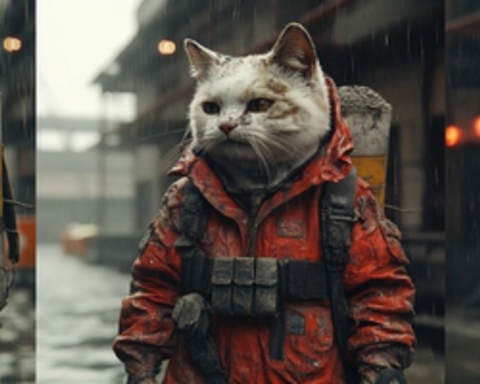
\includegraphics[width=2.660cm,height=2.128cm]{figures/img/subject_tiles/ewmbench.png}}};
\draw[black!35,line width=0.35pt] (2.770,-7.476) rectangle (5.430,-9.604);
\node[anchor=north west,text=ACMDarkBlue,font=\scriptsize,inner sep=0] at (2.790,-9.624) {\href{https://arxiv.org/abs/2505.09694}{EWMBench}};
\node[anchor=north west,text=black!55,font=\tiny,inner sep=0] at (2.790,-9.854) {\href{https://arxiv.org/abs/2505.09694}{arXiv:2505.09694}};
\node[anchor=north west,inner sep=0] at (5.480,-7.476) {\href{https://arxiv.org/abs/2501.09038}{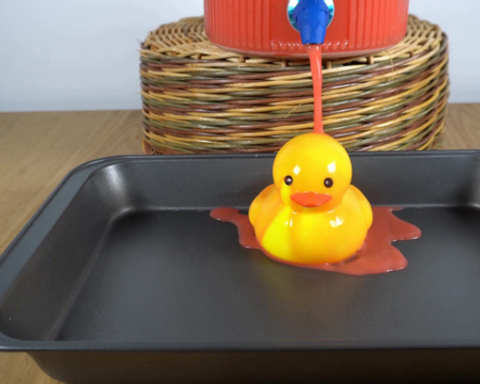
\includegraphics[width=2.660cm,height=2.128cm]{figures/img/subject_tiles/physicsiq.png}}};
\draw[black!35,line width=0.35pt] (5.480,-7.476) rectangle (8.140,-9.604);
\node[anchor=north west,text=ACMDarkBlue,font=\scriptsize,inner sep=0] at (5.500,-9.624) {\href{https://arxiv.org/abs/2501.09038}{Physics-IQ}};
\node[anchor=north west,text=black!55,font=\tiny,inner sep=0] at (5.500,-9.854) {\href{https://arxiv.org/abs/2501.09038}{arXiv:2501.09038}};
\node[anchor=north west,inner sep=0] at (8.190,-7.476) {\href{https://arxiv.org/abs/2106.08261}{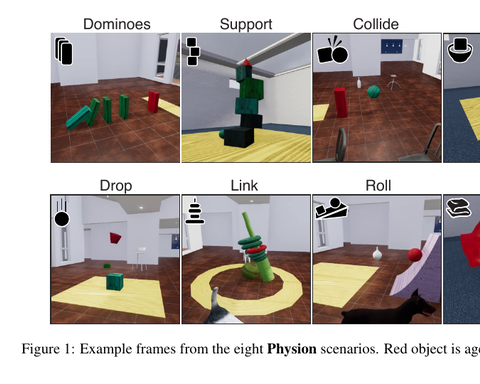
\includegraphics[width=2.660cm,height=2.128cm]{figures/img/subject_tiles/physion.png}}};
\draw[black!35,line width=0.35pt] (8.190,-7.476) rectangle (10.850,-9.604);
\node[anchor=north west,text=ACMDarkBlue,font=\scriptsize,inner sep=0] at (8.210,-9.624) {\href{https://arxiv.org/abs/2106.08261}{Physion}};
\node[anchor=north west,text=black!55,font=\tiny,inner sep=0] at (8.210,-9.854) {\href{https://arxiv.org/abs/2106.08261}{arXiv:2106.08261}};
\node[anchor=north west,inner sep=0] at (10.900,-7.476) {\href{https://arxiv.org/abs/2306.15668}{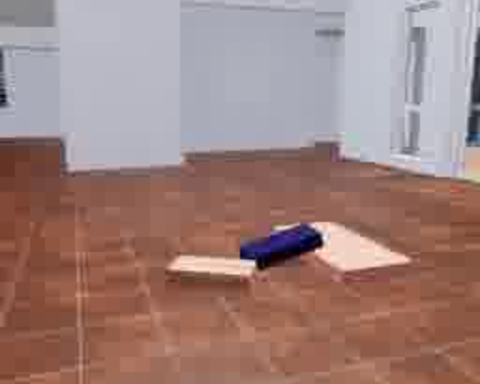
\includegraphics[width=2.660cm,height=2.128cm]{figures/img/subject_tiles/physionpp.png}}};
\draw[black!35,line width=0.35pt] (10.900,-7.476) rectangle (13.560,-9.604);
\node[anchor=north west,text=ACMDarkBlue,font=\scriptsize,inner sep=0] at (10.920,-9.624) {\href{https://arxiv.org/abs/2306.15668}{Physion++}};
\node[anchor=north west,text=black!55,font=\tiny,inner sep=0] at (10.920,-9.854) {\href{https://arxiv.org/abs/2306.15668}{arXiv:2306.15668}};
\node[anchor=north west,inner sep=0] at (0.060,-10.234) {\href{https://arxiv.org/abs/2406.03520}{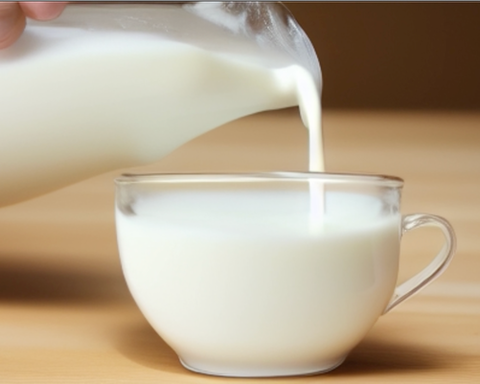
\includegraphics[width=2.660cm,height=2.128cm]{figures/img/subject_tiles/videophy.png}}};
\draw[black!35,line width=0.35pt] (0.060,-10.234) rectangle (2.720,-12.362);
\node[anchor=north west,text=ACMDarkBlue,font=\scriptsize,inner sep=0] at (0.080,-12.382) {\href{https://arxiv.org/abs/2406.03520}{VideoPhy}};
\node[anchor=north west,text=black!55,font=\tiny,inner sep=0] at (0.080,-12.612) {\href{https://arxiv.org/abs/2406.03520}{arXiv:2406.03520}};
\node[anchor=north west,inner sep=0] at (2.770,-10.234) {\href{https://arxiv.org/abs/2502.20694}{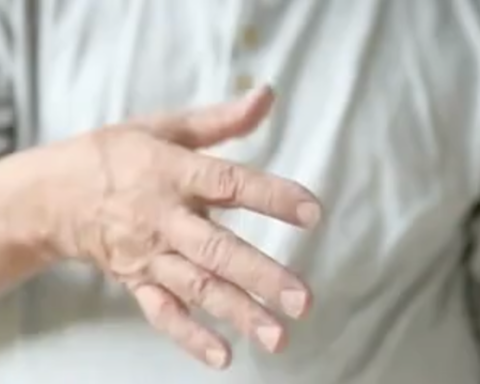
\includegraphics[width=2.660cm,height=2.128cm]{figures/img/subject_tiles/worldmodelbench.png}}};
\draw[black!35,line width=0.35pt] (2.770,-10.234) rectangle (5.430,-12.362);
\node[anchor=north west,text=ACMDarkBlue,font=\scriptsize,inner sep=0] at (2.790,-12.382) {\href{https://arxiv.org/abs/2502.20694}{WorldModelBench}};
\node[anchor=north west,text=black!55,font=\tiny,inner sep=0] at (2.790,-12.612) {\href{https://arxiv.org/abs/2502.20694}{arXiv:2502.20694}};
\node[anchor=north west,inner sep=0] at (5.480,-10.234) {\href{https://arxiv.org/abs/2504.00983}{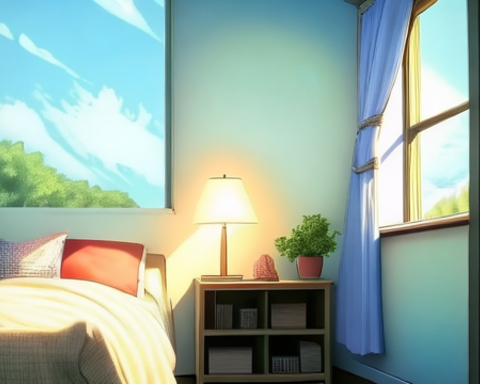
\includegraphics[width=2.660cm,height=2.128cm]{figures/img/subject_tiles/worldscore.png}}};
\draw[black!35,line width=0.35pt] (5.480,-10.234) rectangle (8.140,-12.362);
\node[anchor=north west,text=ACMDarkBlue,font=\scriptsize,inner sep=0] at (5.500,-12.382) {\href{https://arxiv.org/abs/2504.00983}{WorldScore}};
\node[anchor=north west,text=black!55,font=\tiny,inner sep=0] at (5.500,-12.612) {\href{https://arxiv.org/abs/2504.00983}{arXiv:2504.00983}};
\node[anchor=north west,inner sep=0] at (8.190,-10.234) {\href{https://arxiv.org/abs/2503.21755}{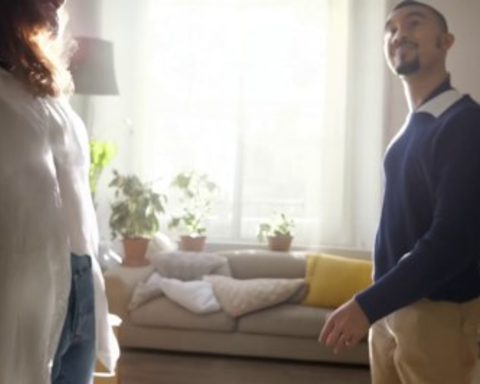
\includegraphics[width=2.660cm,height=2.128cm]{figures/img/subject_tiles/vbench20.png}}};
\draw[black!35,line width=0.35pt] (8.190,-10.234) rectangle (10.850,-12.362);
\node[anchor=north west,text=ACMDarkBlue,font=\scriptsize,inner sep=0] at (8.210,-12.382) {\href{https://arxiv.org/abs/2503.21755}{VBench-2.0}};
\node[anchor=north west,text=black!55,font=\tiny,inner sep=0] at (8.210,-12.612) {\href{https://arxiv.org/abs/2503.21755}{arXiv:2503.21755}};
\node[anchor=north west,inner sep=0] at (10.900,-10.234) {\href{https://arxiv.org/abs/2506.04363}{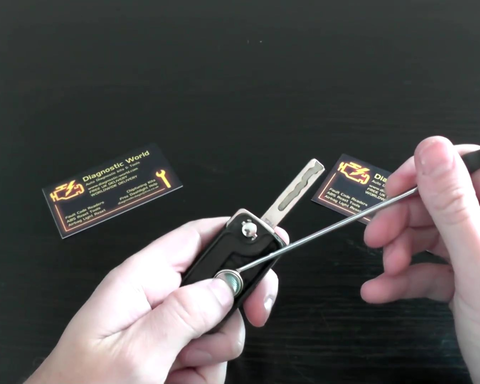
\includegraphics[width=2.660cm,height=2.128cm]{figures/img/subject_tiles/worldprediction.png}}};
\draw[black!35,line width=0.35pt] (10.900,-10.234) rectangle (13.560,-12.362);
\node[anchor=north west,text=ACMDarkBlue,font=\scriptsize,inner sep=0] at (10.920,-12.382) {\href{https://arxiv.org/abs/2506.04363}{WorldPrediction}};
\node[anchor=north west,text=black!55,font=\tiny,inner sep=0] at (10.920,-12.612) {\href{https://arxiv.org/abs/2506.04363}{arXiv:2506.04363}};
\fill[sgBridge!78!black] (0,-13.092) rectangle (13.80,-13.592);
\node[anchor=west,text=white,font=\footnotesize\bfseries,inner sep=0] at (0.12,-13.342) {PREDICTION-TO-ACTION bridges};
\node[anchor=north west,inner sep=0] at (0.060,-13.662) {\href{https://arxiv.org/abs/2410.18072}{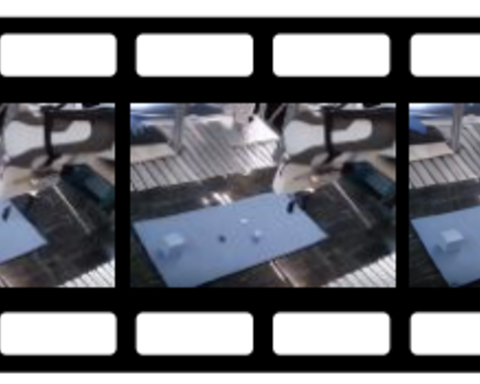
\includegraphics[width=2.660cm,height=2.128cm]{figures/img/subject_tiles/worldsimbench.png}}};
\draw[black!35,line width=0.35pt] (0.060,-13.662) rectangle (2.720,-15.790);
\node[anchor=north west,text=ACMDarkBlue,font=\scriptsize,inner sep=0] at (0.080,-15.810) {\href{https://arxiv.org/abs/2410.18072}{WorldSimBench}};
\node[anchor=north west,text=black!55,font=\tiny,inner sep=0] at (0.080,-16.040) {\href{https://arxiv.org/abs/2410.18072}{arXiv:2410.18072}};
\node[anchor=north west,inner sep=0] at (2.770,-13.662) {\href{https://arxiv.org/abs/2510.18135}{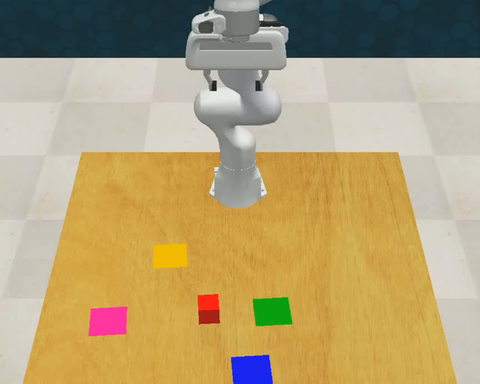
\includegraphics[width=2.660cm,height=2.128cm]{figures/img/subject_tiles/worldinworld.png}}};
\draw[black!35,line width=0.35pt] (2.770,-13.662) rectangle (5.430,-15.790);
\node[anchor=north west,text=ACMDarkBlue,font=\scriptsize,inner sep=0] at (2.790,-15.810) {\href{https://arxiv.org/abs/2510.18135}{World-in-World}};
\node[anchor=north west,text=black!55,font=\tiny,inner sep=0] at (2.790,-16.040) {\href{https://arxiv.org/abs/2510.18135}{arXiv:2510.18135}};
\node[anchor=north west,inner sep=0] at (5.480,-13.662) {\href{https://arxiv.org/abs/2604.19092}{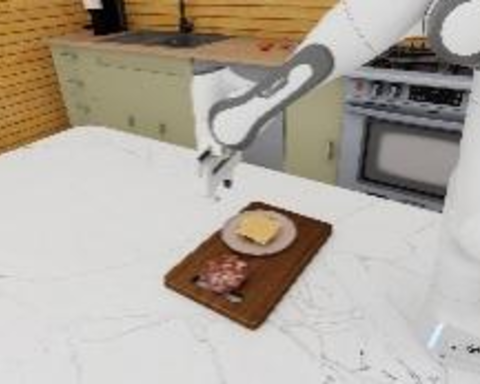
\includegraphics[width=2.660cm,height=2.128cm]{figures/img/subject_tiles/robowmbench.png}}};
\draw[black!35,line width=0.35pt] (5.480,-13.662) rectangle (8.140,-15.790);
\node[anchor=north west,text=ACMDarkBlue,font=\scriptsize,inner sep=0] at (5.500,-15.810) {\href{https://arxiv.org/abs/2604.19092}{RoboWM-Bench}};
\node[anchor=north west,text=black!55,font=\tiny,inner sep=0] at (5.500,-16.040) {\href{https://arxiv.org/abs/2604.19092}{arXiv:2604.19092}};
\node[anchor=north west,inner sep=0] at (8.190,-13.662) {\href{https://arxiv.org/abs/2602.08971}{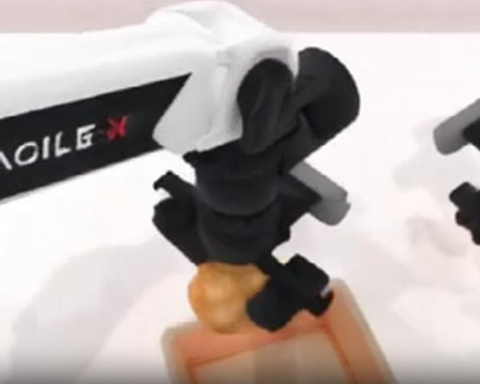
\includegraphics[width=2.660cm,height=2.128cm]{figures/img/subject_tiles/worldarena.png}}};
\draw[black!35,line width=0.35pt] (8.190,-13.662) rectangle (10.850,-15.790);
\node[anchor=north west,text=ACMDarkBlue,font=\scriptsize,inner sep=0] at (8.210,-15.810) {\href{https://arxiv.org/abs/2602.08971}{WorldArena}};
\node[anchor=north west,text=black!55,font=\tiny,inner sep=0] at (8.210,-16.040) {\href{https://arxiv.org/abs/2602.08971}{arXiv:2602.08971}};
\end{tikzpicture}}
\caption{\textbf{Benchmarks across the surveyed corpus.} Representative subject figures from the catalogue, grouped by evaluation lane rather than embodiment: \emph{closed-loop} task-success suites, \emph{open-loop} world-model and video-generation evaluation, and the \emph{prediction-to-action bridges}. Each panel is a live hyperlink to the source paper on arXiv and is annotated with its arXiv id (per-panel figure provenance in Table~\ref{tab:panel_provenance}); the figure is vector with photographs embedded at full resolution, so it can be zoomed without pixelation. Only figures that depict the benchmark's task or scene are shown; results and leaderboard figures appear in Figure~\ref{fig:results_gallery}. Benchmarks with no locatable subject figure are omitted, not fabricated. Images \textcopyright\ their respective authors, reproduced for scholarly review.}
\Description{A gallery of benchmark subject figures in three lane bands. The top band, closed-loop task-success suites, shows ten policy and embodied benchmark scenes (robot arms and simulated households). The middle band, open-loop world-model and video-generation evaluation, shows ten generated-video or physical-scene samples. The bottom band, prediction-to-action bridges, shows four world-model benchmark scenes. Each panel is labelled with the benchmark name and its arXiv id.}
\label{fig:subject_gallery}
\end{figure*}
